\documentclass{beamer}
\usetheme{McMaster}
\beamertemplatenavigationsymbolsempty 
\usepackage{tikz}
\usepackage[export]{adjustbox} % for left/right justifying images
\title{ChatGPT, procedural generation, and large language models: a history}
\author{John Fink}

% Talk is 2023-05-25 1pm.
% ideas / outline
% Randomness
	% e.g. coin flips
% I-Ching and PKD
% Bibliomancy
% That homework machine book
% Bryon Gysin / WSB cut-up
% Markov chaining
% ELIZA
% oblique strategies?
% that 1980s Racter thing and Policeman's Beard
% Demo racter in archive.org 
% Rogue and roguelikes
% https://github.com/brexhq/prompt-engineering is EXCELLENT for history and terms and stuff.
% N-gram models (markov chains; demonstrate dadadodo)
% ChatGPT (sigh)
% Labour issues
% 	IBM outsourcing
% Important LLM (including ChatGPT concepts)
%	context size
%	parameters (7b, 13b, 30b, 65b)
%	Training (Lora, RLHF, few-shot, zero-shot) 
%	Temperature and those other llama.cpp variables (which I think are
%	common to all LLMs)
%	The Prompt
% Other proprietary LLMs (slightly less exasperated sigh)
%	Bard? Anthropic? BERT/RoBERTa?
% Open Source LLMs
% 	Meta's LLaMa
% 	LlaMa Leak
%	Hugging Face
%	Everything else!!!!
%	Non-LLaMa models
% 		StarCoder, RedPajama, etc. etc. etc.
%	Two ways to run local
%		CPU vs GPU
% 		emphasize that CPU is *many factors slower* than GPU
%	Demo llama.cpp
% 	EU's AI act? 
\begin{document}
\begin{frame}
    \maketitle
\end{frame}

\begin{frame}
	John Fink
	
	Digital Scholarship Librarian
	
	McMaster University
\end{frame}

% LAND ACQ HERE: 
% 

% McMaster University stands on the traditional territory shared between the Haudenosaunee  confederacy and the Anishinabe nations. This territory is covered by the Upper Canada Treaties, is within the lands protected by the “Dish With One Spoon” wampum agreement and is directly adjacent to Haldiman Treaty territory.

% We must acknowledge a debt to those who were here before us, and recognize our responsibility, as guests, to respect and honour the intimate relationship Indigenous peoples have to this land. 


\begin{frame}
	A (series of) disclaimers:
\end{frame}
 
 % Disclaimers: procrastination (for a reason), English major, many many demos, and randomness in those demos. No idea what's going to be said or anything. Will address ChatGPT but it is not at all the point of the talk generally.

 \begin{frame}[plain]
 	\makebox[\linewidth]{
\includegraphics[width=\paperwidth,height=\paperheight]{dontknow}}
 \end{frame}

 \begin{frame}
 	What is \textit{randomness}?
 \end{frame}

\begin{frame}[c]
	\centering
	\Huge
	Yijing / I-Ching
	
	(1000-750 BC)
\end{frame}
  
  % Wikipedia: s a divination text, the I Ching is used for a traditional Chinese form of cleromancy known as I Ching divination, in which bundles of yarrow stalks are manipulated to produce sets of six apparently random numbers ranging from 6 to 9. Each of the 64 possible sets corresponds to a hexagram, which can be looked up in the I Ching. The hexagrams are arranged in an order known as the King Wen sequence. The interpretation of the readings found in the I Ching has been endlessly discussed and debated over the centuries. Many commentators have used the book symbolically, often to provide guidance for moral decision-making, as informed by Confucianism, Taoism and Buddhism. 
  
  \begin{frame}[plain]
  	\makebox[\linewidth]{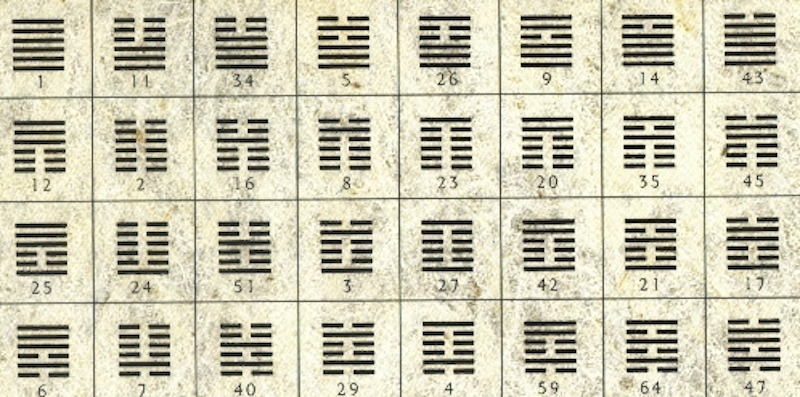
\includegraphics[width=\paperwidth,height=\paperheight]{i-ching.jpg}}
  \end{frame}
  \begin{frame}[c]
  	\centering
  	\Huge
  	The Man in the High Castle
  	
  	(1962)
  \end{frame}

% Wiki: Throughout the story, the characters make important decisions based upon their interpretations of prophetic messages from the I Ching, a Chinese book of divination.

\begin{frame}[plain]
	\makebox[\linewidth]{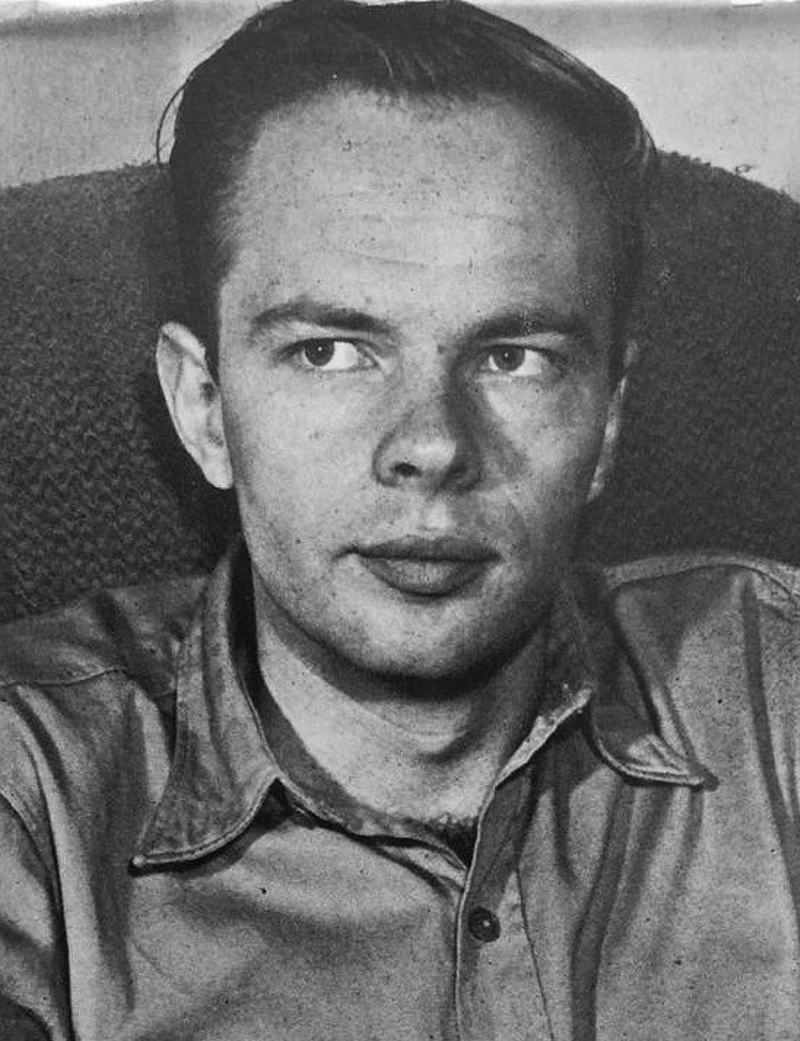
\includegraphics[height=\paperheight]{pkd.jpg}}
\end{frame}

% As a novelist, Dick used the I Ching to craft the themes, plot and story of The Man in the High Castle, whose characters also use the I Ching to inform and guide their decisions.

\begin{frame}[c]
	\centering
	\Huge
	Bibliomancy
	
	(1753 - as a term)
\end{frame}

\begin{frame}[plain]
	\makebox[\linewidth]{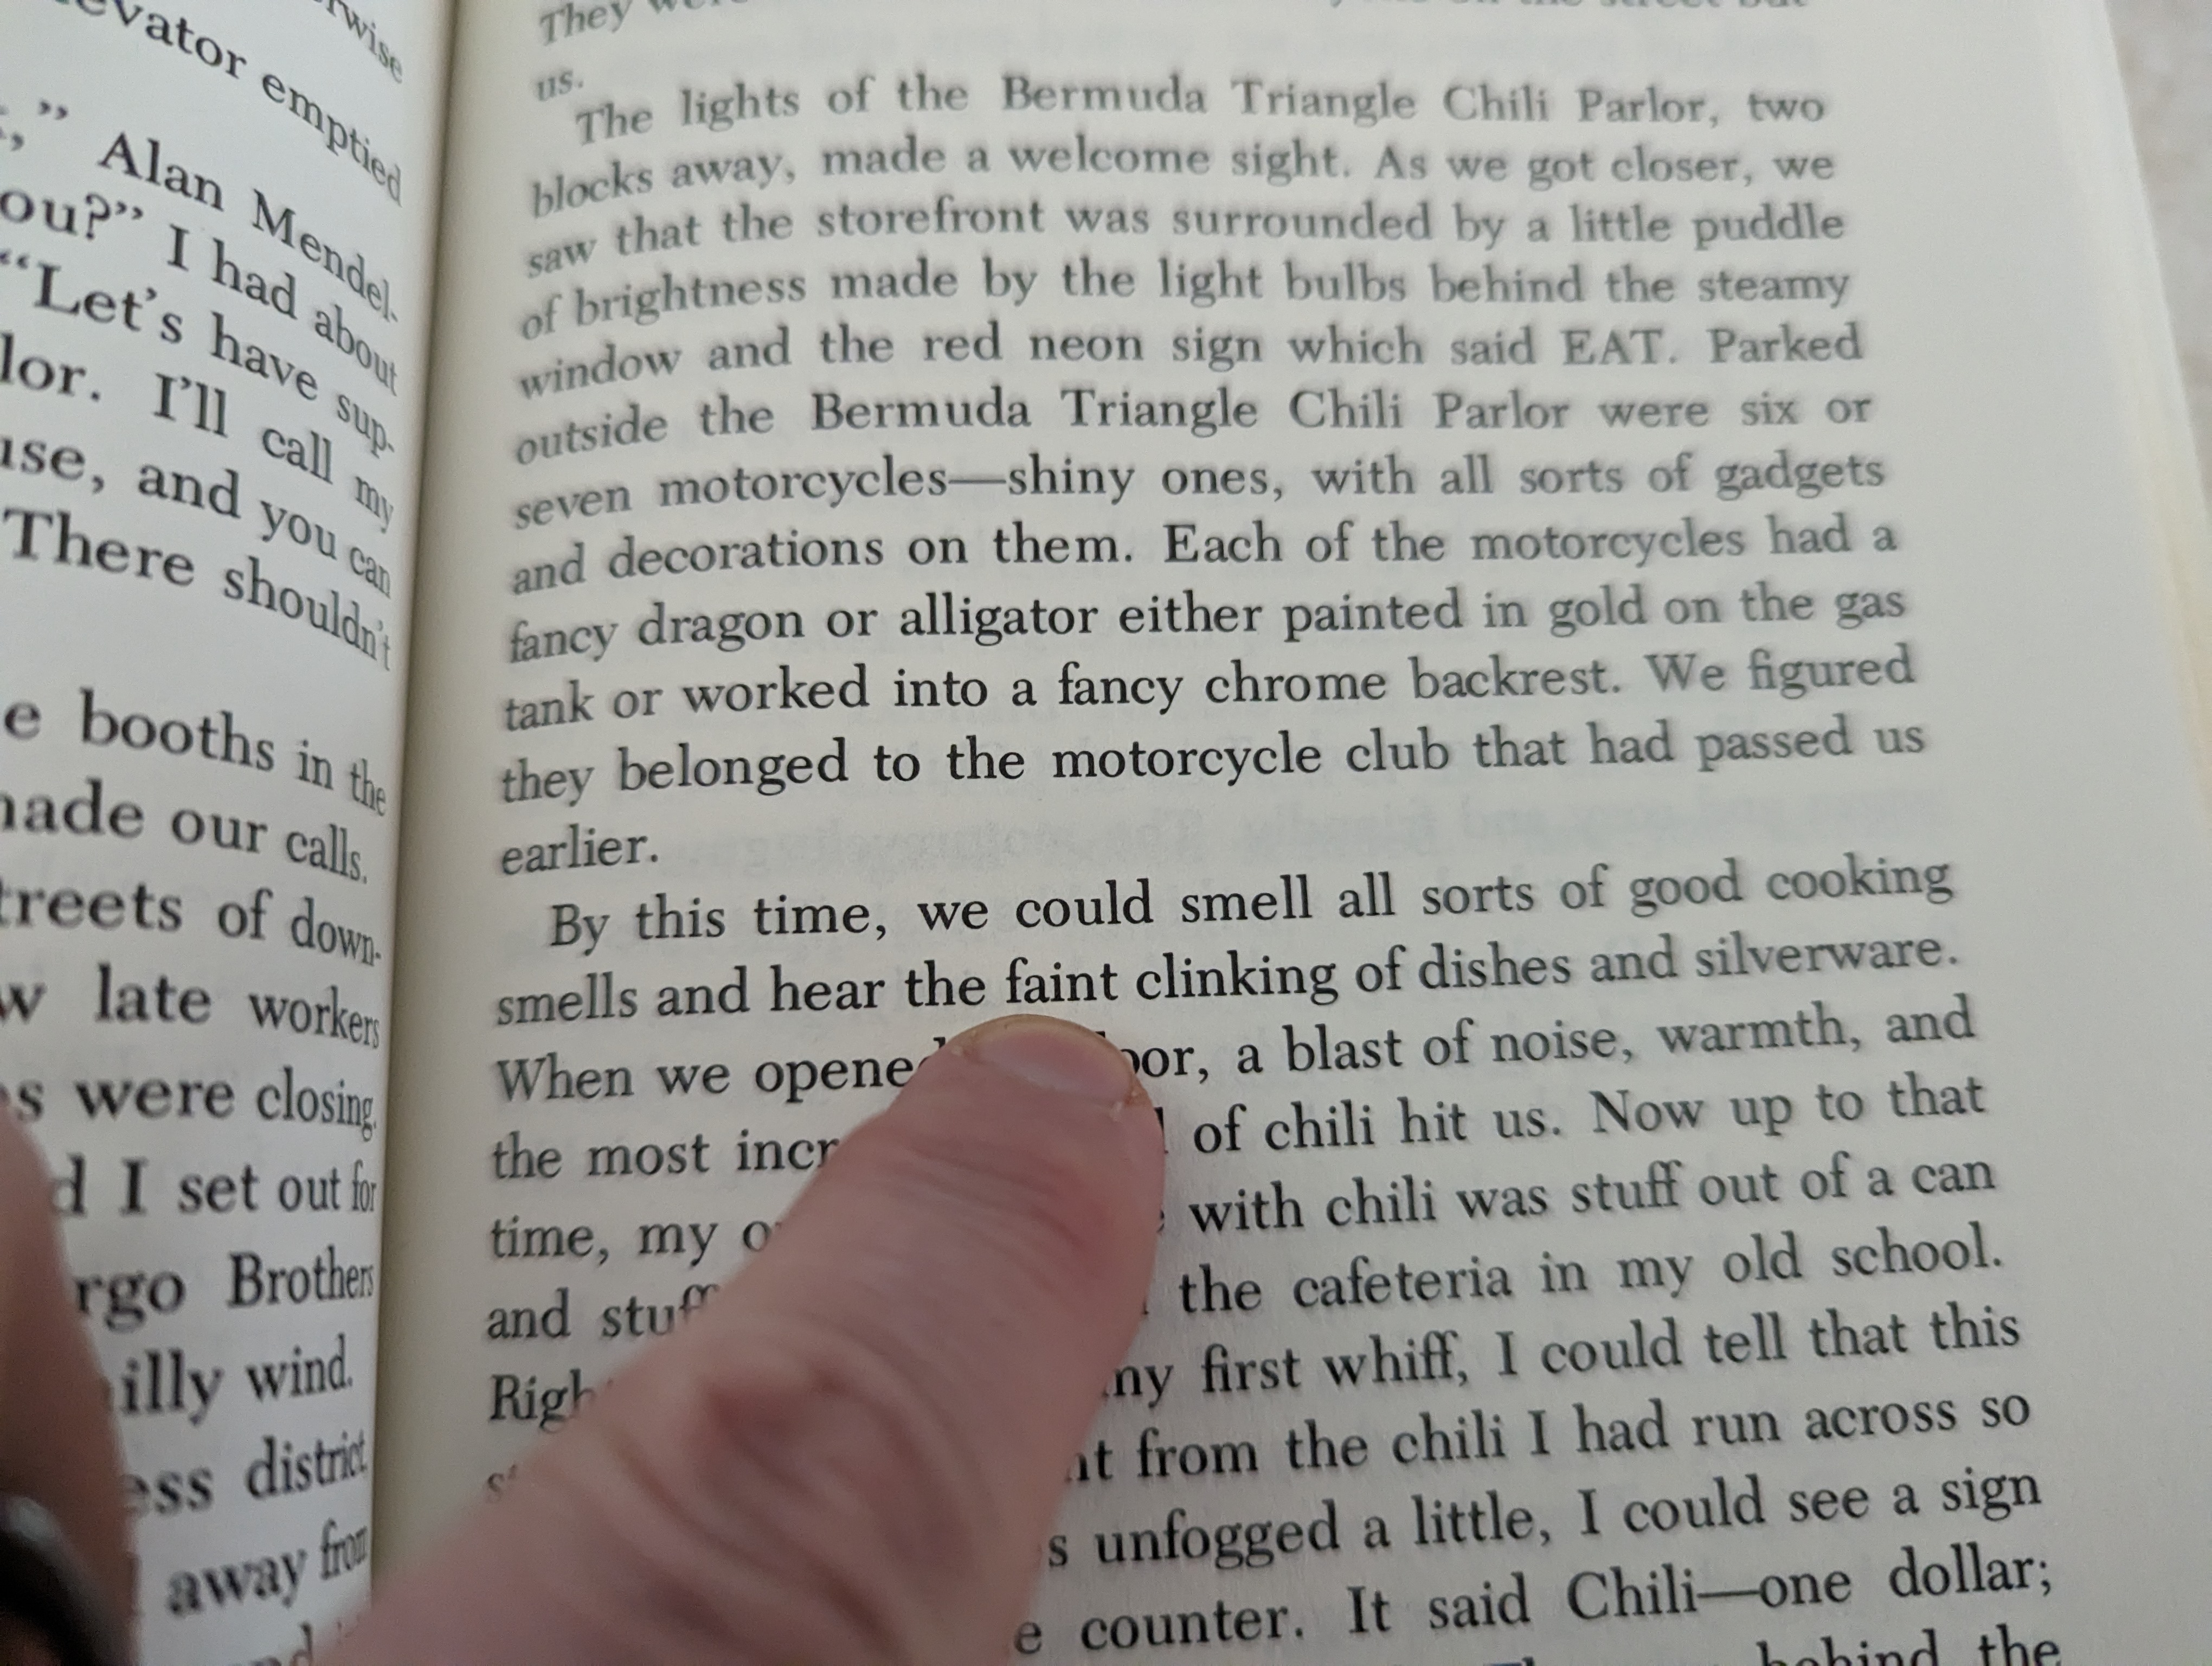
\includegraphics[width=\paperwidth,height=\paperheight]{pinkwater-bibliomancy.jpg}}
\end{frame}

%		A book is picked that is believed to hold truth.
%		It is balanced on its spine and allowed to fall open.
%		A passage is picked, with the eyes closed.
%		Usually done with a religious book.

\begin{frame}[c]
	\centering
	\Huge
	The Cut-Up Technique
	
	(1920s)
\end{frame}


\begin{frame}[plain]
	\makebox[\linewidth]{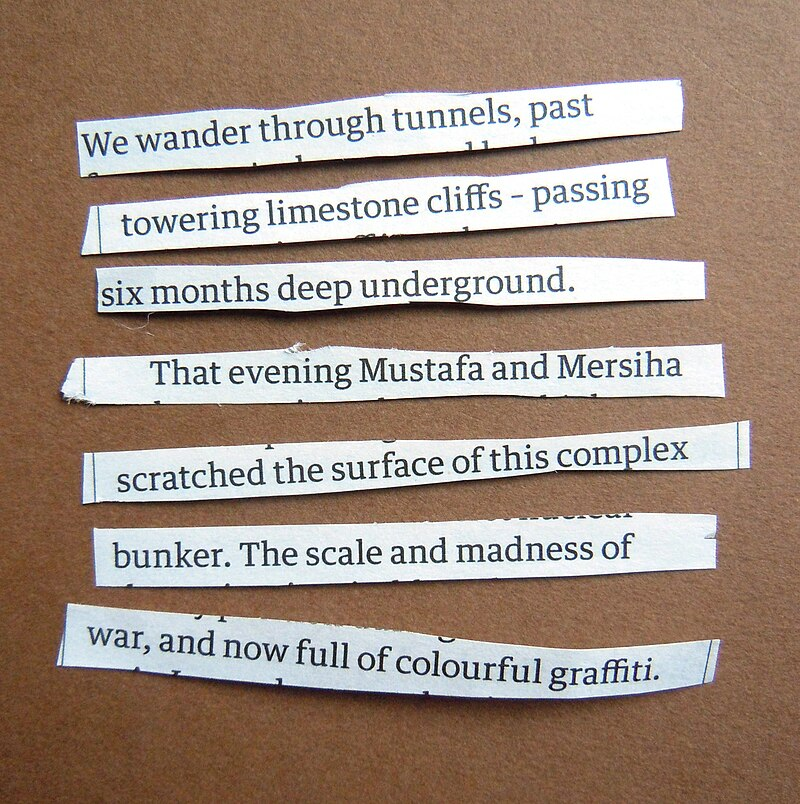
\includegraphics[width=\paperwidth,height=\paperheight]{cut-up.jpg}}
\end{frame}

% Started by the Dadaists in the 1920s but reached more exposure in the 1950s and 1960s with Canadian poet Brion Gysin and William S. Burroughs. 

\begin{frame}[c]
	\centering
	\Huge
	ELIZA
	
	(1966)
\end{frame}

\begin{frame}[plain]
	\makebox[\linewidth]{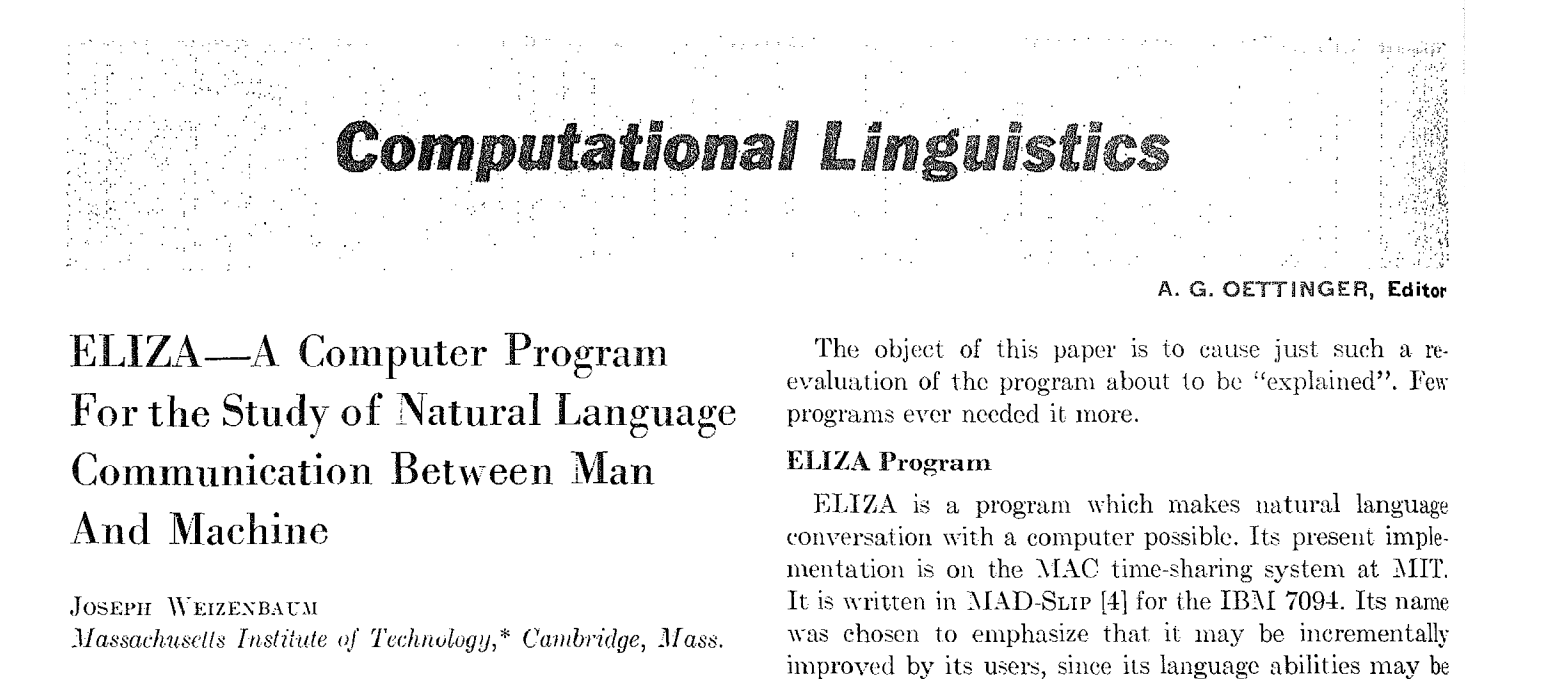
\includegraphics[width=\paperwidth,height=\paperheight]{eliza-paper}}
\end{frame}

\begin{frame}[c]
	\centering
	\Huge
	Oblique Strategies
	
	(1975)
\end{frame}

\begin{frame}[plain]
	\makebox[\linewidth]{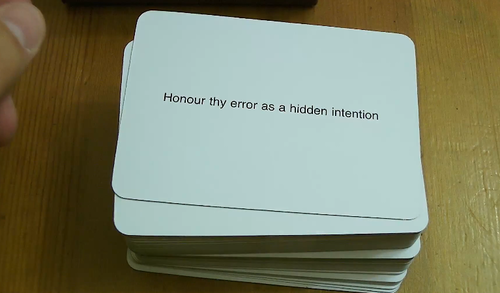
\includegraphics[width=\paperwidth,height=\paperheight]{oblique}}
\end{frame}

\begin{frame}[c]
	\centering
	\Huge
	Rogue
	
	(1980)
\end{frame}

\begin{frame}[plain]
	\makebox[\linewidth]{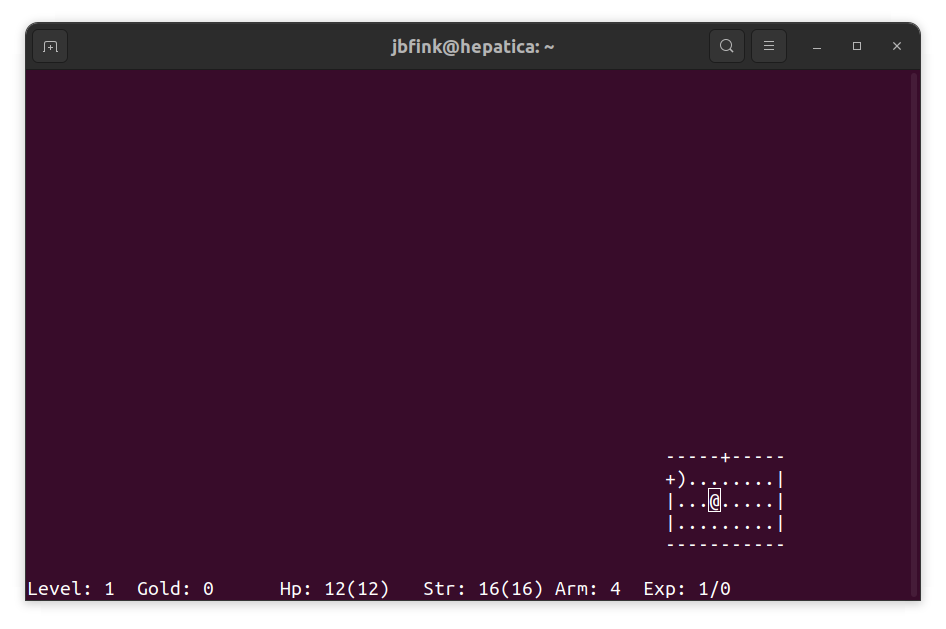
\includegraphics[width=\paperwidth,height=\paperheight]{rogue}}
\end{frame}

\begin{frame}[c]
	\centering
	\Huge
	Murder on the Zinderneuf
	
	(1983)
\end{frame}

\begin{frame}[plain]
	\makebox[\linewidth]{
\includegraphics[width=\paperwidth,height=\paperheight]{zinderneuf}}
\end{frame}

\begin{frame}[plain]
	\makebox[\linewidth]{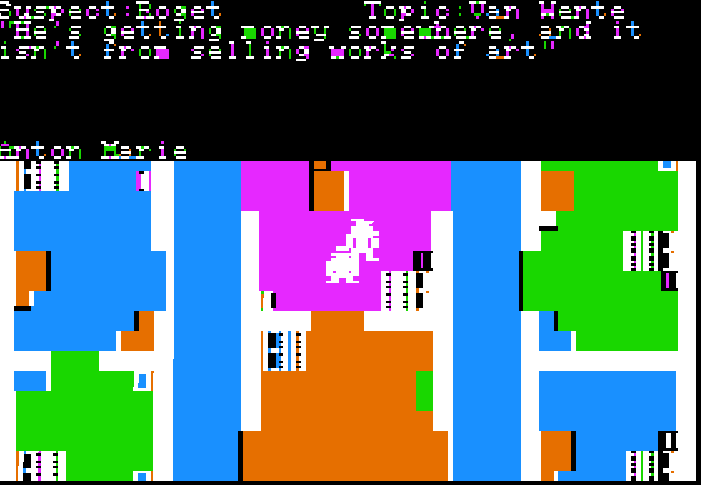
\includegraphics[width=\paperwidth,height=\paperheight]{zinderneuf2}}
\end{frame}

\begin{frame}[c]
	\centering
	\Huge
	Racter and The Policeman's Beard
	
	(1984)
\end{frame}

\begin{frame}[plain]
	\makebox[\linewidth]{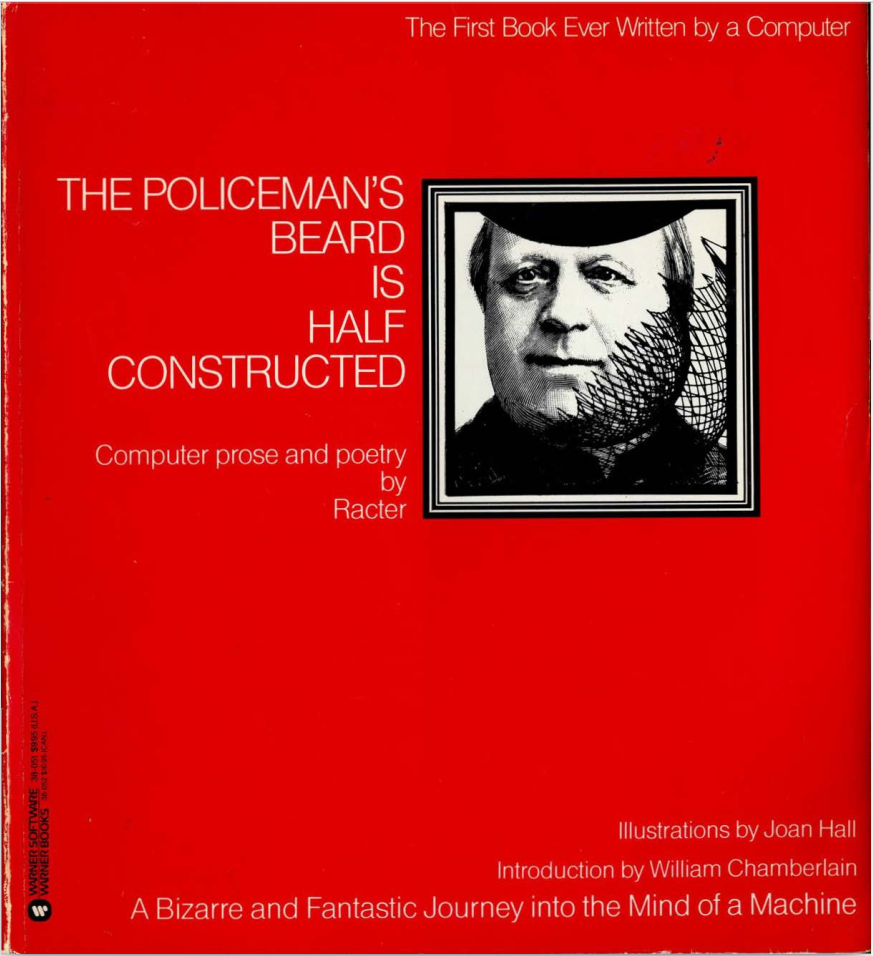
\includegraphics[height=\paperheight]{policemans-beard}}
\end{frame}

\begin{frame}[plain]
	\makebox[\linewidth]{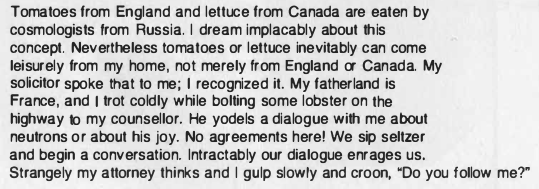
\includegraphics[width=\paperwidth,height=\paperheight]{beard-sample}}
\end{frame}

% racter demo here -- run in Chrome: run https://archive.org/details/msdos_Racter_1984

%The 1958 / Danny Dunn thing should probably go right before you actually talk about LLMs

\begin{frame}{so, to recap:}
	\begin{itemize}
		\item 1000BC - Yijing / I-Ching
		\pause
		\item 1000BC-2017AD - some inconsequential stuff happens
	\end{itemize}
\end{frame}

\begin{frame}[c]
	but wait!
	
	\centering
	\Huge
	Danny Dunn and the Homework Machine
	
	(1958)
\end{frame}

\begin{frame}[plain]
	\makebox[\linewidth]{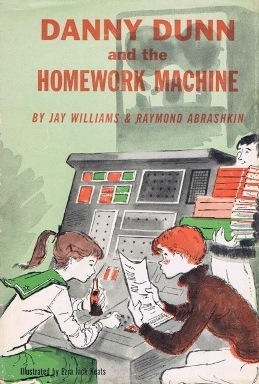
\includegraphics[height=\paperheight]{dannydunn.jpg}}
\end{frame}

\begin{frame}
	A little conversation about the weather.
\end{frame}

\begin{frame}[plain]
	\makebox[\linewidth]{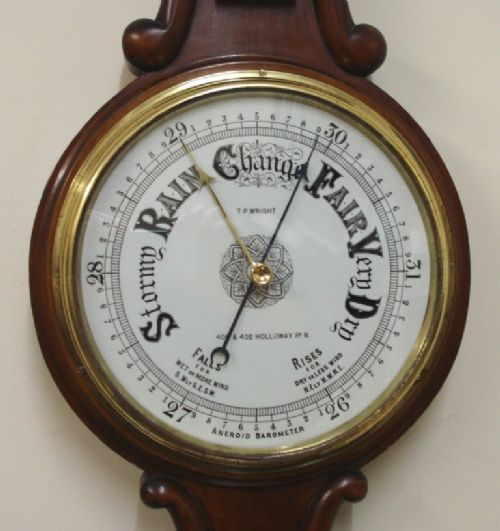
\includegraphics[width=\paperwidth,height=\paperheight]{barometer}}
\end{frame}

\begin{frame}[plain]
	\makebox[\linewidth]{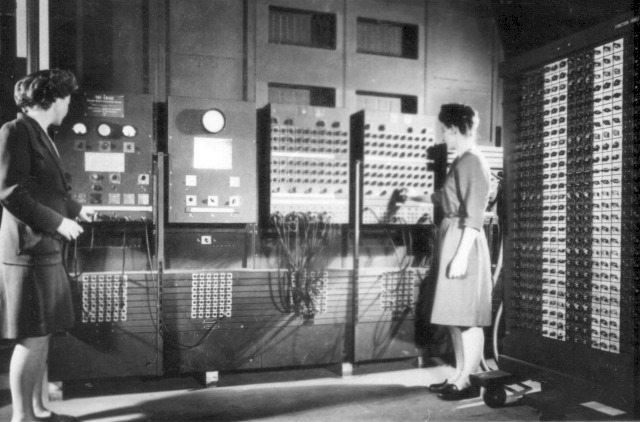
\includegraphics[width=\paperwidth,height=\paperheight]{eniac}}
\end{frame}


\begin{frame}
	Why I say "Large Language Model" and not "AI"
\end{frame}


% SPECIAL CODE WORD HERE: HAL


\begin{frame}
	So, about 2017...
\end{frame}

\begin{frame}[plain]
	\makebox[\linewidth]{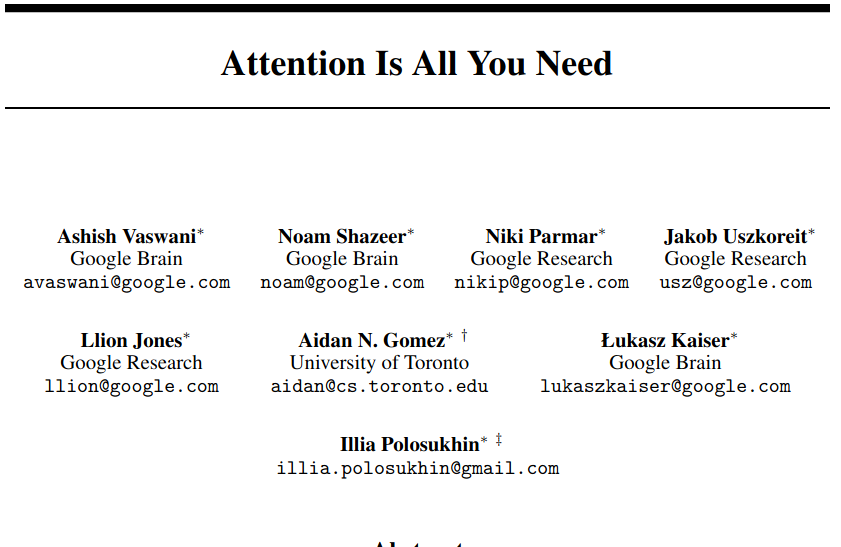
\includegraphics[width=\paperwidth,height=\paperheight]{attention}}
\end{frame}

\begin{frame}{2017-now! Right now!}
	\begin{itemize}
		\item 2017 - "Attention Is All You Need" paper
		\pause
		\item 2018 - "Improving Language Understanding by Generative Pre-Training" paper
		\pause 
		\item 2020 - "Language Models are Few-Shot Learners" paper (GPT-3)
		\pause
		\item 2022 - InstructGPT, and then ChatGPT
		\pause
		\item 2023 - and then....
	\end{itemize}
\end{frame}

\begin{frame}[plain]
	\makebox[\linewidth]{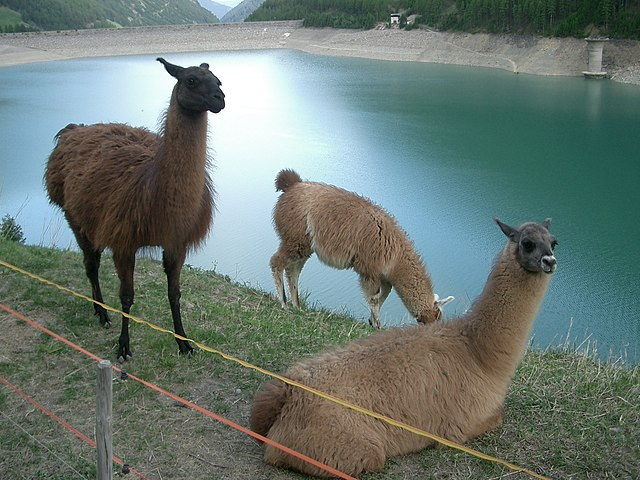
\includegraphics[width=\paperwidth,height=\paperheight]{llamas}}
\end{frame}

\begin{frame}
	"Progress is now moving so swiftly that every few weeks the state-of-the-art is changing or models that previously required clusters to run now run on Raspberry PIs."
	 
	 -- https://github.com/brexhq/prompt-engineering
\end{frame}

\begin{frame}{Important concepts for GPT and other models}
	\begin{itemize}
		\item Context Window and Tokens
		% 2k for LLaMa, 4k for GPT4 chat, 8k/32k via API. This is short term memory.
		\pause
		\item Few-Shot / No-Shot
		\pause
		\item Parameters
		% GPT-1 117m, GPT-2 1.5b, GPT-3 175b, GPT-4 170t 
		\pause
		\item The Prompt, aka "Programming for English Majors"
		\pause
		\item And the Random Seed.
	\end{itemize}
\end{frame}

\begin{frame}
	\begin{itemize}
		\item Context Window is the "memory" of an LLM
		\pause
		\item And Tokens -- words, roughly -- fill up that "memory"
		\pause
		\item And the \textit{response} also takes tokens.
	\end{itemize}
\end{frame}

% demo https://platform.openai.com/tokenizer

\begin{frame}[plain]
	\makebox[\linewidth]{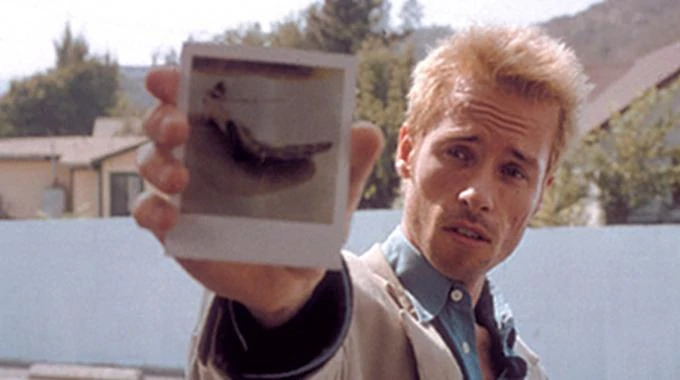
\includegraphics[width=\paperwidth,height=\paperheight]{leonard}}
\end{frame}

\begin{frame}{Few-Shot / No-Shot}
	\begin{itemize}
		\item \textit{Few-Shot} -- a few examples to "teach" an LLM, such as:
		\pause
		\item "I hate it when my phone battery dies." - negative
		\pause
		\item "My day has been great!" - positive
		\pause
		\item "Here is an article." - neutral
		\pause
		\item "This presentation is going fantastic!!!!" - positive
		\pause
		\item And \textit{No-Shot} is exactly what you think it is.
	\end{itemize}
\end{frame}


\begin{frame}{Parameters}
	\begin{itemize}
		\item Roughly corresponds to how "Complex" or "Smart" a model is.
		\pause
		\item (...very roughly)
		\pause 
		\item But \textit{definitely} correlates to resources needed to run the model.
		\pause
		\item Which is why, say, GPT-4 requires this....
	\end{itemize}
\end{frame}

\begin{frame}[plain]
	\makebox[\linewidth]{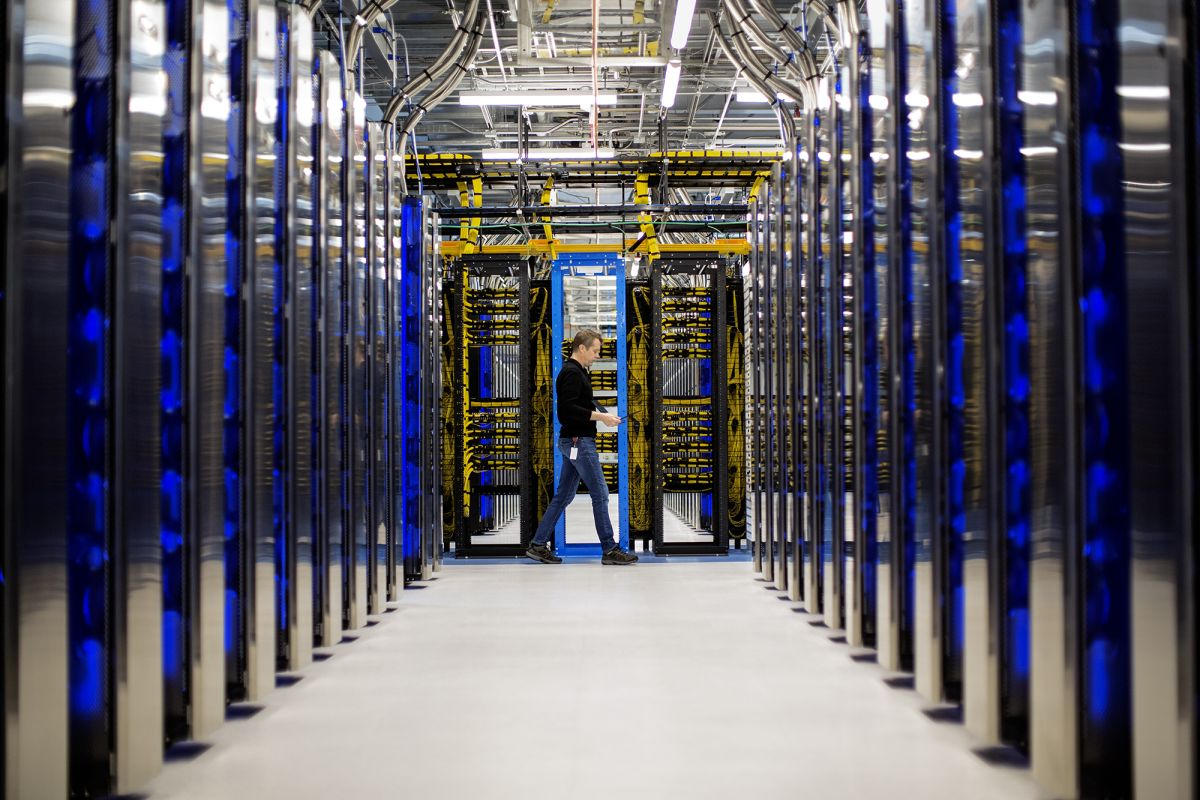
\includegraphics[width=\paperwidth,height=\paperheight]{azure-data-centre}}
\end{frame}

\begin{frame}
	And you can run a 7B model on this....
\end{frame}

\begin{frame}[plain]
	\makebox[\linewidth]{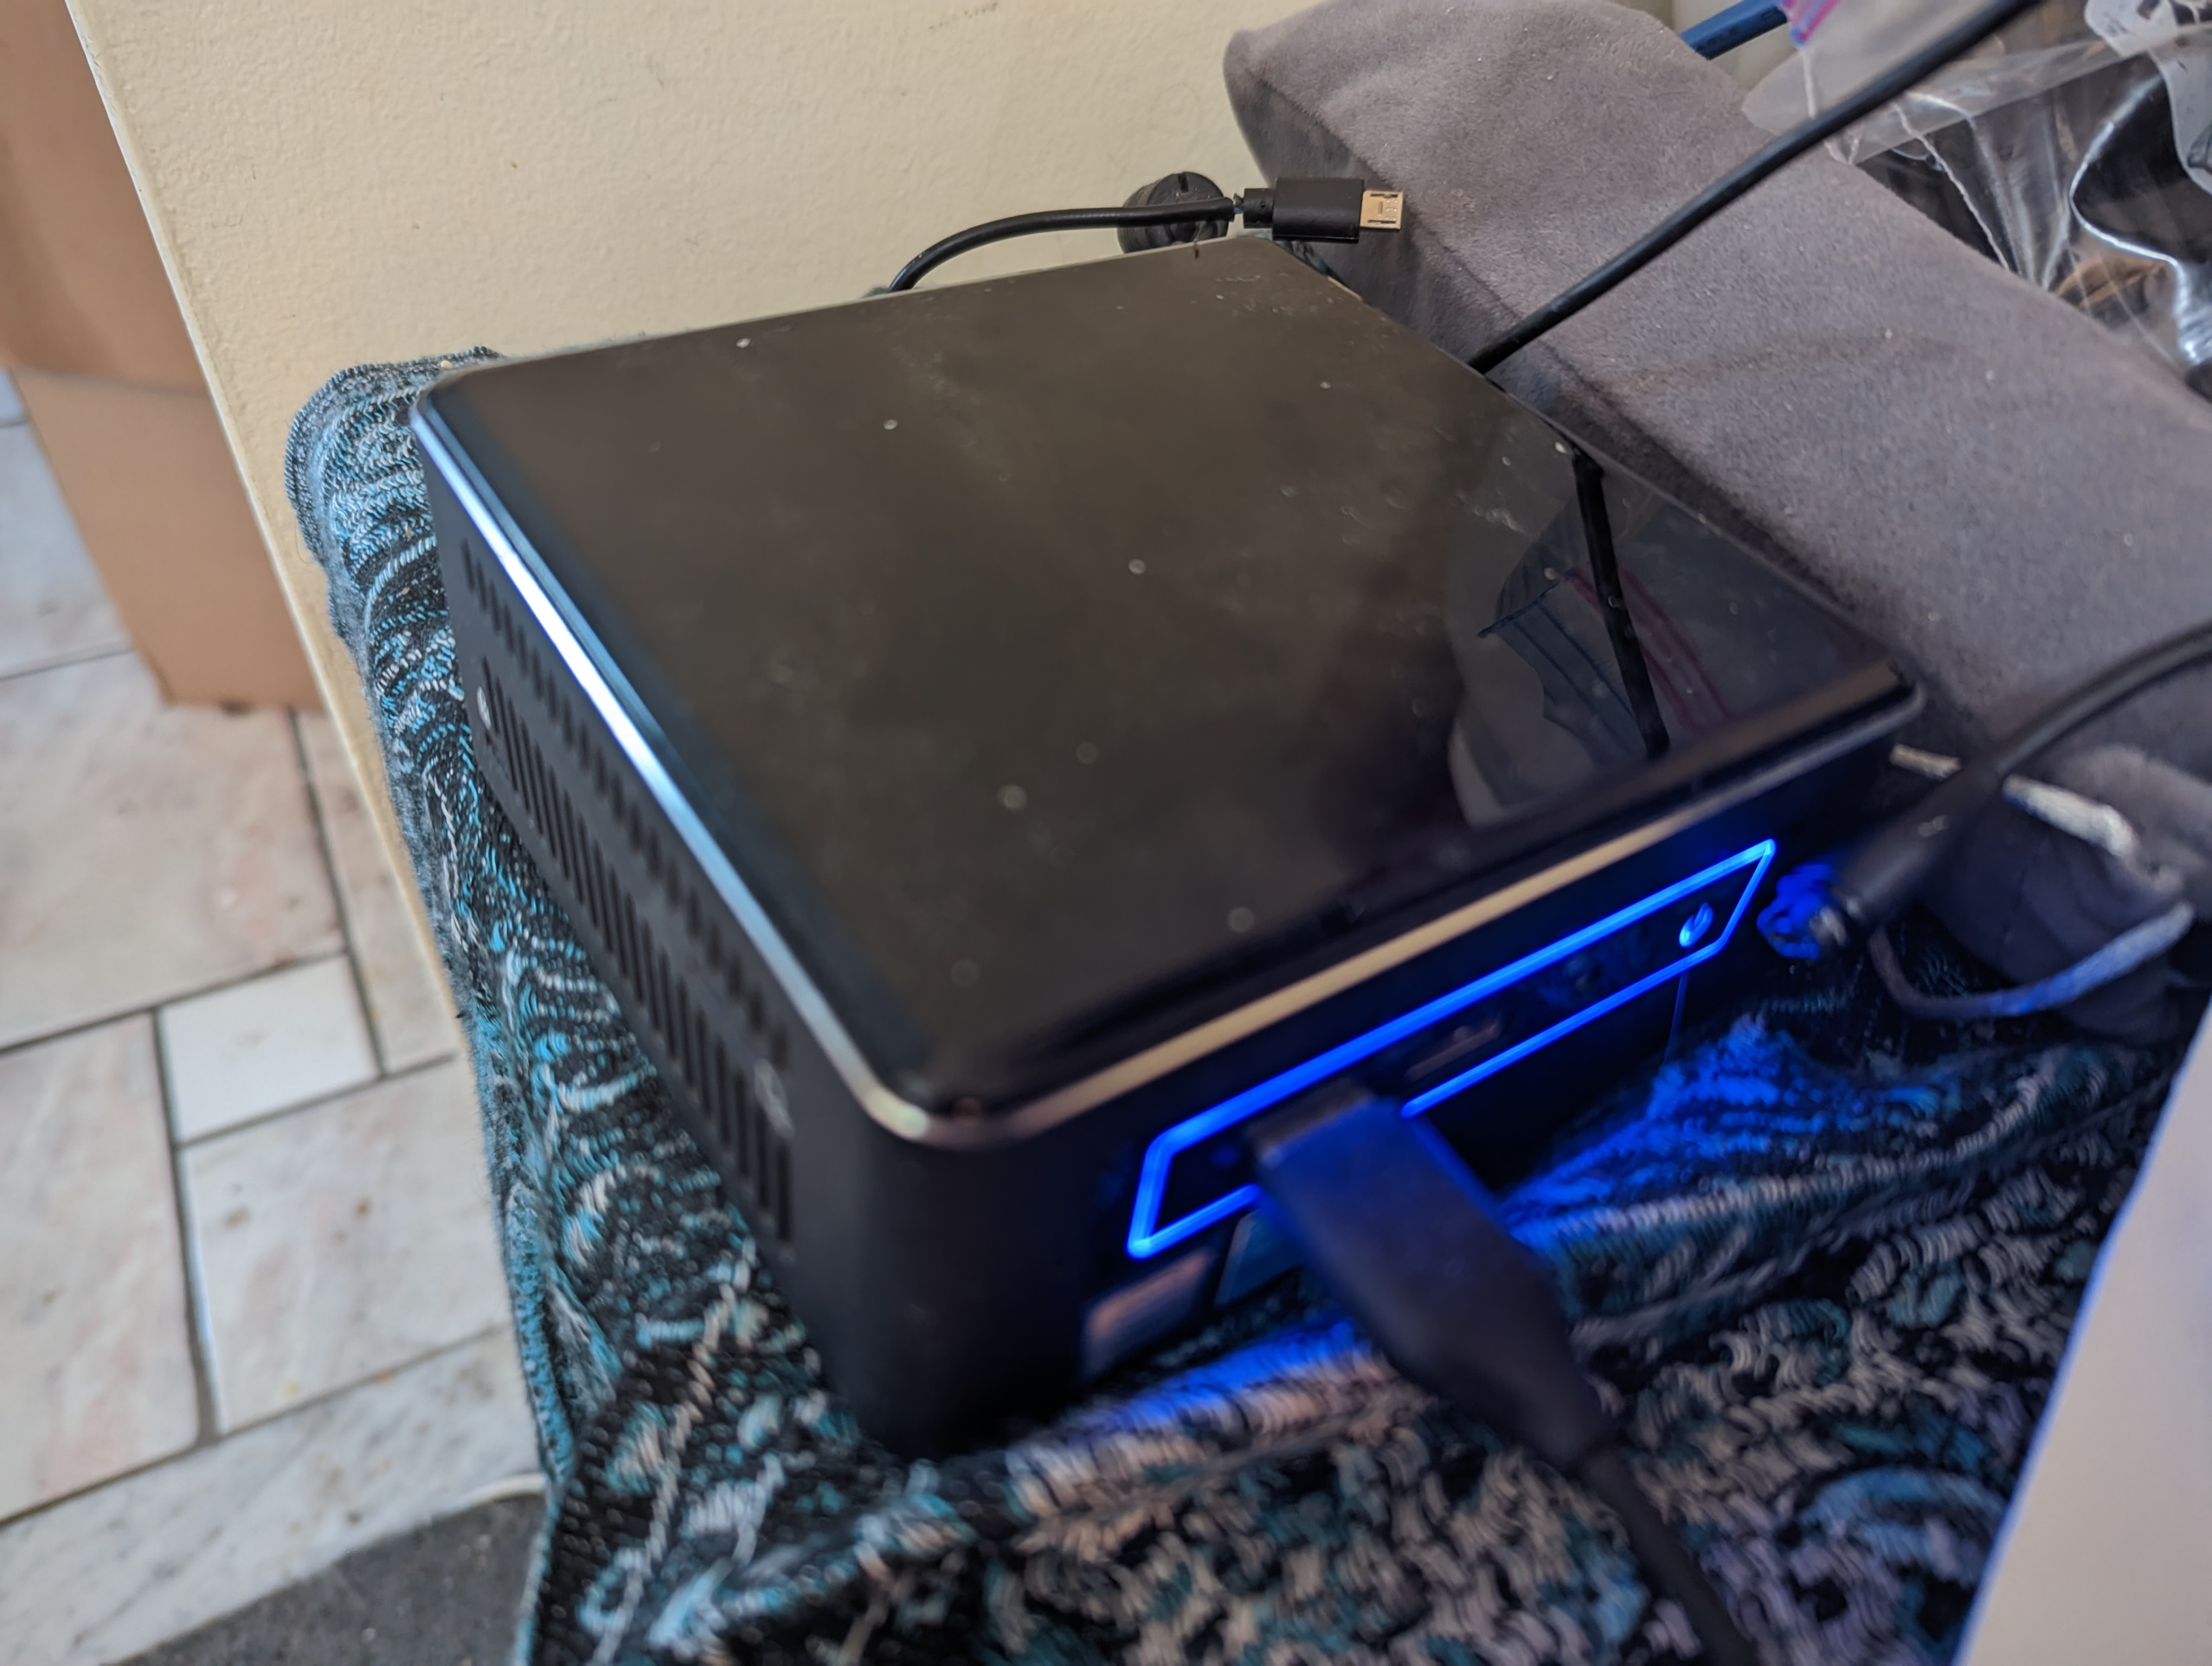
\includegraphics[width=\paperwidth,height=\paperheight]{pfeebe}}
\end{frame}


\begin{frame}
	llama.cpp -- https://github.com/ggerganov/llama.cpp
\end{frame}


% demo soup-to-nuts build of llama.cpp on pfeebe:
% git clone https://github.com/ggerganov/llama.cpp
% make clean; make LLAMA_OPENBLAS=1
% copy model file 
% Demo librarian.txt -- have it make up APA references for John Fink and then ask it the two apples / one banana logic problem
% Demo huggingface.co/chat
% also demo privateGPT if you have time.

% move this slide to *just* before you actually talk about LLMs.


\begin{frame}{We Have No Moat}
	In May (yes, the month that we are still in right now) a Google internal document was leaked to the public, titled "We Have No Moat, and Neither Does OpenAI". It's worth quoting some bits from it, because it's a doozy.
\end{frame}

\begin{frame}{We Have No Moat}
	\begin{itemize}
		\item "While our models still hold a slight edge in terms of quality, the gap is closing astonishingly quickly. Open-source models are faster, more customizable, more private, and pound-for-pound more capable. They are doing things with \$100 and 13B params that we struggle with at \$10M and 540B. And they are doing so in weeks, not months. This has profound implications for us."
		\pause
		\item "Indeed, in terms of engineer-hours, the pace of improvement from these models vastly outstrips what we can do with our largest variants, and the best are already largely indistinguishable from ChatGPT. Focusing on maintaining some of the largest models on the planet actually puts us at a disadvantage."
	\end{itemize}
\end{frame}

\begin{frame}{THE FUTURE OF LARGE LANGUAGE MODELS}
	\begin{itemize}
		\item ....Skynet????
		\pause
		\item ....fully automated luxury communism???
		\pause 
		\item ....larger context windows?
		
	\end{itemize}
	
	
	
\end{frame}

\begin{frame}
	%this is always the last slide
	Any questions?\\ 
	jfink@mcmaster.ca\\
	
\includegraphics[left, height=4mm]{mastodon} \hspace{1mm}  https://glammr.us/@jbfink
	
\end{frame}

\end{document}
